%%%%%%%%%%%%%%%%%%%%%%%%%%%%%%%%%%%%%%%%%%%%%%%%%%%
%																													
%																												
%																													
%									Importations	de bibliothèques	
%																													
%																												
%%%%%%%%%%%%%%%%%%%%%%%%%%%%%%%%%%%%%%%%%%%%%%%%%%%


\documentclass[hidelinks]{article}
\usepackage[utf8]{inputenc}
\usepackage{graphicx}
\usepackage[T1]{fontenc}
\usepackage[french]{babel}
\usepackage{csquotes}
\usepackage[section]{placeins}
\usepackage{tikz}
\usepackage{hyperref}
\usepackage{afterpage}
\usepackage{pdfpages}
\usepackage{wrapfig}
\usepackage{amsmath, mathtools}
\usepackage{amssymb}
\usepackage{fancyhdr}
\usepackage[all]{background}


%%%%%%%%%%%%%%%%%%%%%%%%%%%%%%%%%%%%%%%%%%%%%%%%%%%%%%%%%%%%%%%%%%%%
%																																	   %
%																																	   %
%																																	   %
%															Page de garde															   %
%																																	   %
%																																	   %
%%%%%%%%%%%%%%%%%%%%%%%%%%%%%%%%%%%%%%%%%%%%%%%%%%%%%%%%%%%%%%%%%%%%



\newcommand{\MyGraphicLogo}{% For imported graphic logo
\begin{tikzpicture}[remember picture,overlay,yshift=-15cm, xshift=10.5cm]
	\definecolor{gris}{RGB}{16,52,78}
	\definecolor{jaune_fonce}{RGB}{0, 107, 163}
	\definecolor{jaune}{RGB}{0, 151, 136}
	\fill [gris] (-10.5,-10) -- (0,-4.5) -- (14,-13) -- (14,-16)--(0,-16)--(-10.5,-16);
	\fill [jaune_fonce] (0,-4.5) -- (-10.5,-10) -- (-10.5, 1.8);
	\node at (3.8,0.4) {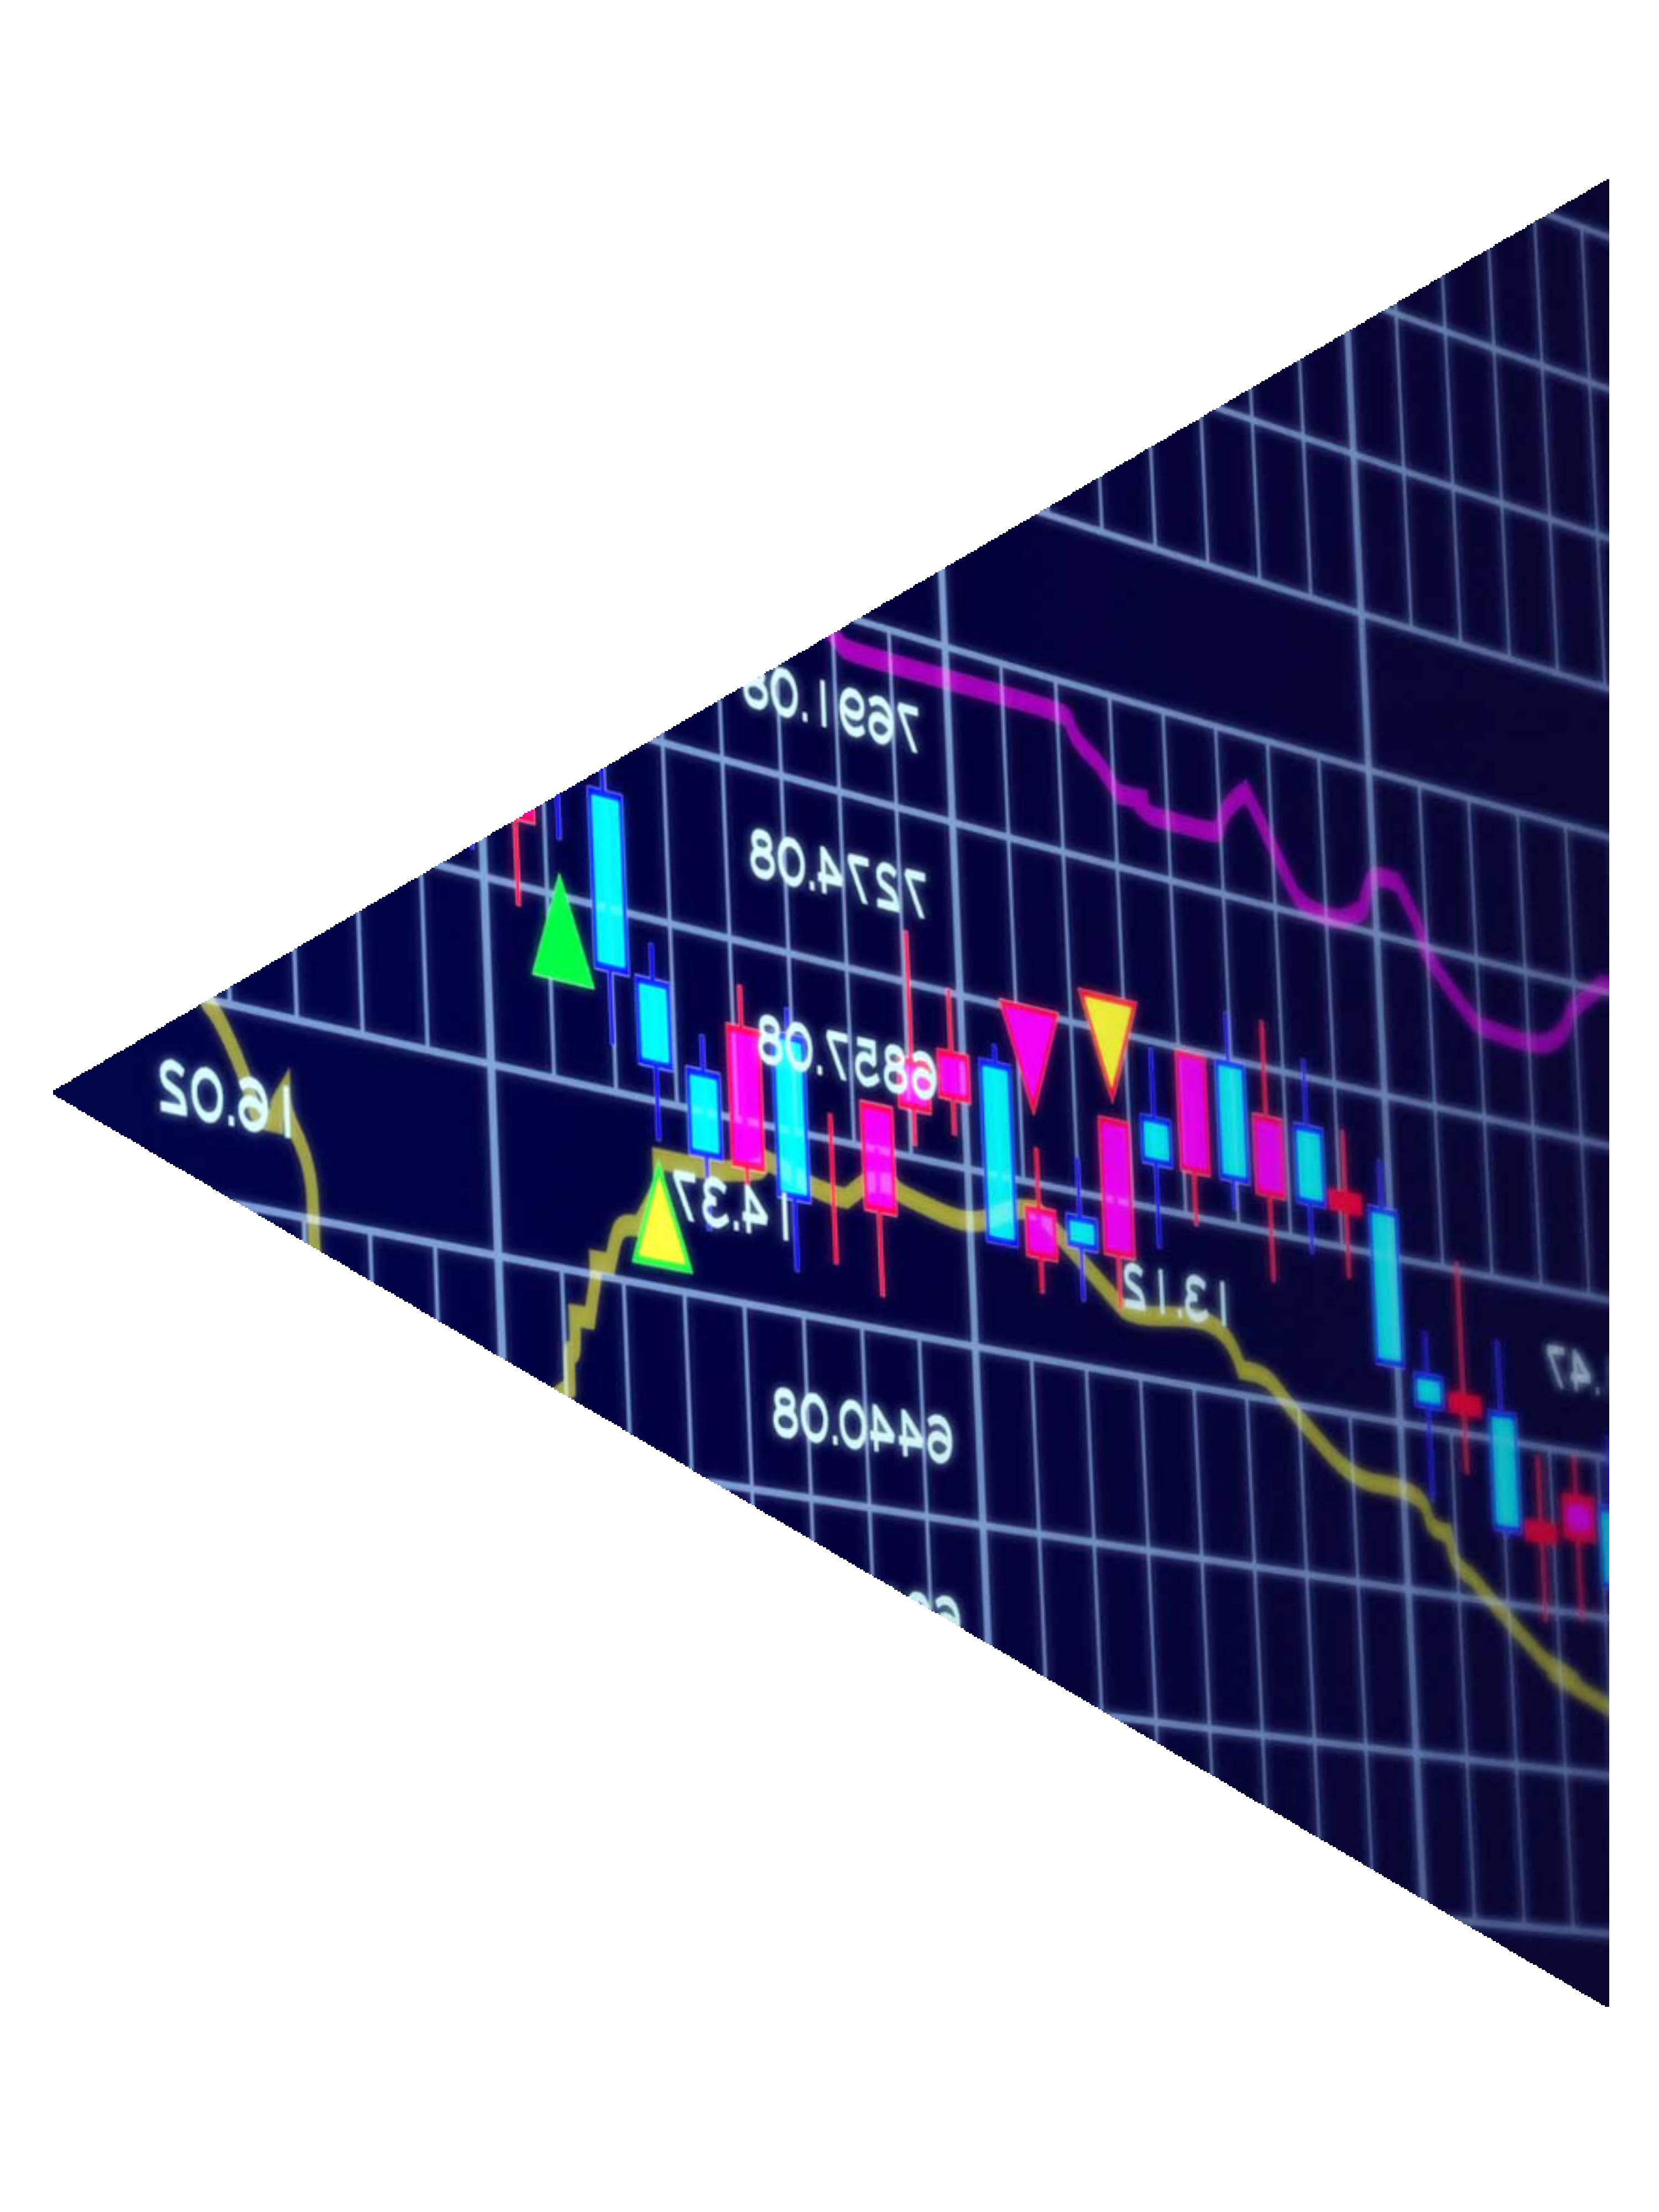
\includegraphics[width=22cm]{triangle.png}};
	\fill [jaune] (14,5) -- (2.5, 12) -- (20,25) -- (14, 20);
 \end{tikzpicture}}


\SetBgContents{\MyGraphicLogo}% Select included image

\SetBgPosition{current page.north west}% Select location
\SetBgOpacity{1.0}% Select opacity
\SetBgAngle{0.0}% Select roation of logo
\SetBgScale{1.0}% Select scale factor of logo



%%%%%%%%%%%%%%%%%%%%%%%%%%%%%%%%%%%%%%%%%%%%%%%%%%%%%%%%%%%%%%%%%%%%
%																																	   %
%																																	   %
%																																	   %
%										Informations générales sur le document															   %
%																																	   %
%																																	   %
%%%%%%%%%%%%%%%%%%%%%%%%%%%%%%%%%%%%%%%%%%%%%%%%%%%%%%%%%%%%%%%%%%%%

 \usepackage{fontspec}
  \usepackage[bold-style=upright]{unicode-math}
  \defaultfontfeatures{Scale=1}
  \setmainfont[Ligatures=TeX,Numbers=OldStyle]{Lucida Bright OT}
  \setmathfont[RawFeature=+ss04]{Lucida Bright Math OT}
  \setsansfont[Scale=1.0,Numbers=OldStyle]{Myriad Pro}
  \newfontfamily\fullcaps[Letters=Uppercase,Numbers=Uppercase]{Myriad Pro}
  \usepackage[babel=true]{microtype}
  \usepackage{icomma}
  
  
  
  
  
  
  
  
  
  
  
\title{Black-Scholes Formula}
\author{Maxence COUPET - \href{mailto:maxence.coupet@gmail.com}{maxence.coupet@gmail.com}}
\date{March 2018}



\newcommand{\esp}{\mathbb{E}\left[e^{-rT}(S_{T}-K)^{+}\right]}
\newcommand{\dd}{\frac{ln\left(\frac{K}{S_{0}}\right)-\left(r-\frac{\sigma^{2}}{2}\right) T}{\sigma}}
\newcommand{\ddd}{\frac{ln\left(\frac{K}{S_{0}}\right)-\left(r-\frac{\sigma^{2}}{2}\right) T}{\sigma \sqrt{T}}}
\newcommand{\dddd}{\frac{ln\left(\frac{S_{0}}{K}\right)+\left(r-\frac{\sigma^{2}}{2}\right) T}{\sigma \sqrt{T}}}
\newcommand{\ddddd}{\frac{ln\left(\frac{K}{S_{0}}\right)-\left(r-\frac{\sigma^{2}}{2}\right) T}{\sigma \sqrt{T}}-\sigma\sqrt{T}}
\newcommand{\dddddd}{\frac{ln\left(\frac{S_{0}}{K}\right)+\left(r+\frac{\sigma^{2}}{2}\right) T}{\sigma \sqrt{T}}}
\newcommand*{\QEDB}{\hfill\ensuremath{\square}}


\MHInternalSyntaxOn
\MH_set_boolean_T:n {outer_mult}
\MHInternalSyntaxOff

\newenvironment{nalign}{
    \begin{equation}
    \begin{aligned}
}{
    \end{aligned}
    \end{equation}
    \ignorespacesafterend
}

%%%%%%%%%%%%%%%%%%%%%%%%%%%%%%%%%%%%%%%%%%%%%%%%%%%%%%%%%%%%%%%%%%%%
%																																	   %
%																																	   %
%																																	   %
%												Mis en page du document																   %
%																																	   %
%																																	   %
%%%%%%%%%%%%%%%%%%%%%%%%%%%%%%%%%%%%%%%%%%%%%%%%%%%%%%%%%%%%%%%%%%%%


\begin{document}
	\selectlanguage{french}
	% page de garde
	\pagenumbering{gobble}
	\maketitle
	\newpage
	% début du rapport
	
	
	


\newcommand{\MyGraphicLog}{% For imported graphic logo
\begin{tikzpicture}[remember picture,overlay,yshift=-15cm, xshift=10.5cm]
\definecolor{jaune}{RGB}{16, 52, 78};
\fill[jaune] (-11, -16) -- (13, -16) -- (13, -12.1) -- (-11, -12.1);
 \end{tikzpicture}}


\SetBgContents{\MyGraphicLog}% Select included image


\SetBgPosition{current page.north west}% Select location
\SetBgOpacity{1.0}% Select opacity
\SetBgAngle{0.0}% Select roation of logo
\SetBgScale{1.0}% Select scale factor of logo

\pagestyle{fancy}
\renewcommand\headrulewidth{0pt}
\lhead{}\chead{}\rhead{}
\cfoot{\vspace*{6\baselineskip} \textcolor{white}{\thepage} \large}
	\newpage

	\pagenumbering{arabic}

%%%%%%%%%%%%%%%%%%%%%%%%%%%%%%%%%%%%%%%%%%%%%%%%%%%%%%%%%%%%%%%%%%%%
%																																	   %
%																																	   %
%																																	   %
%								Début du document (commencez à taper votre texte ici)													   %
%																																	   %
%																																	   %
%%%%%%%%%%%%%%%%%%%%%%%%%%%%%%%%%%%%%%%%%%%%%%%%%%%%%%%%%%%%%%%%%%%%
	
    We want to compute the the fair price for an european call option on a stock which doesn't pay dividends.
    
    
	\section{Hypothesis}
	
	Let the interest rate $r$ and the volatility $\sigma>0$ be constant.
	
	Let the stock price be a geometric Brownian motion (i.e. stock price returns follow a log-normal distribution) : $$\forall t>0, \quad S_{t}=S_{0} \cdot e^{(r - \frac{ \sigma^{2}}{2}) t+\sigma \cdot W_{t}}$$
	whith the initial price $S_{0}>0$ and $(W_{t})_{t>0}$ a Brownian motion, thus $W_{t}\textasciitilde \mathcal{N}(0, t)$.
	
	Let $K>0$ and $T>0$ .
    
    \section{Calculation}
    We will compute $\mathbb{E}\big[e^{-rT}(S_{T}-K)^{+}\big]$ using stochastic integral with respect to the Brownian motion $(W_{t})_{t>0}$ .
    \begin{nalign}
    \esp & = e^{-rT}\int_{\{S_{T}>K\}}^{\infty} \big( S_{T}-K\big) \cdot \frac{e^{-\frac{x^{2}}{2T}}}{\sqrt{2\Pi T}} dx
    \\ & = e^{-rT}\int_{\{S_{T}>K\}}^{\infty} \big( S_{0}e^{(r-\frac{\sigma^{2}}{2})T+\sigma x}-K\big) \cdot \frac{e^{-\frac{x^{2}}{2T}}}{\sqrt{2\Pi T}} dx
    \end{nalign}
    
    In order to determine the integral bound, we make to following caculations :
    \begin{nalign}
    S_{T}>K & \Leftrightarrow ln\left( S_{T} \right)>ln\left( K \right)
    \\  & \Leftrightarrow ln\left( \frac{S_{0}}{K} \right)+\left( r-\frac{\sigma^{2}}{2} \right)T > \sigma 
    \\  & \Leftrightarrow W_{T} > \dd
    \end{nalign}

	We can now replace the bounds :
	\begin{nalign}
    \esp & = e^{-rT}\int_{\dd}^{\infty} \big( S_{T}-K\big) \cdot \frac{e^{-\frac{x^{2}}{2T}}}{\sqrt{2\Pi T}} dx
    \end{nalign}


	Let's use the change of variable $y=\frac{x}{\sqrt{T}} \Rightarrow dy = \frac{dx}{\sqrt{T}}$ :
	\begin{equation}
    \begin{split}
    \esp &= e^{-rT}\int_{\ddd}^{\infty} S_{0} \cdot e^{(r-\frac{\sigma^{2}}{2})T+\sigma \sqrt{T}y} \cdot \frac{e^{-\frac{y^{2}}{2}}}{\sqrt{2\Pi}} dy \\
     &\qquad\qquad - K  e^{-rT}\int_{\ddd}^{\infty} \frac{e^{-\frac{y^{2}}{2}}}{\sqrt{2\Pi}} dy \\
    & = S_{0} \int_{\ddd}^{\infty} \frac{1}{\sqrt{2\Pi}} e^{-\frac{1}{2}\left( y^{2} - 2\sigma\sqrt{T}y + \sigma^{2}T\right)} dy \\ 
   &\qquad\qquad - K  e^{-rT}\int_{\ddd}^{\infty} \frac{e^{-\frac{y^{2}}{2}}}{\sqrt{2\Pi}} dy  \\
     & = S_{0} \int_{\ddd}^{\infty} \frac{1}{\sqrt{2\Pi}} e^{-\frac{1}{2}\left( y - \sigma\sqrt{T}\right)^{2}} dy \\
    & \qquad\qquad- K  e^{-rT}\int_{\ddd}^{\infty} \frac{e^{-\frac{y^{2}}{2}}}{\sqrt{2\Pi}} dy  
    \end{split}
    \end{equation}

We now have to remark that :
\begin{equation}
    \begin{split}
    \int_{a}^{\infty} \frac{1}{\sqrt{2\Pi}}e^{-\frac{y^{2}}{2}} dy & =  \int_{-\infty}^{-a} \frac{1}{\sqrt{2\Pi}}e^{-\frac{y^{2}}{2}} dy 
    \\ & = N(-a)
    \end{split}
    \end{equation}
With $x \mapsto N(x)$ the cumulative standard normal distribution fonction. We have :
\begin{nalign}
    \esp & = S_{0} \int_{\ddd}^{\infty} \frac{1}{\sqrt{2\Pi}} e^{-\frac{1}{2}\left( y - \sigma\sqrt{T}\right)^{2}} dy
    \\ & \qquad\qquad - K  e^{-rT}\int_{-\infty}^{\dddd} \frac{e^{-\frac{y^{2}}{2}}}{\sqrt{2\Pi}} dy 
    \end{nalign}
    
    Let's use the change of variable $\xi=y-\sigma\sqrt{T} \Rightarrow d\xi=dy$ :
    \begin{equation}
    \begin{split}
    \esp & = S_{0} \int_{\ddddd}^{\infty} \frac{1}{\sqrt{2\Pi}} e^{-\frac{\xi^{2}}{2}} d\xi
    \\ & \qquad\qquad - K  e^{-rT}N\left( \dddd \right)
    \end{split}
    \end{equation}
    
    \newpage
    Using again the transformation with the bounds of the integral, we have :
    \begin{equation}
    \begin{split}
    \esp & = S_{0} \int_{-\infty}^{\dddddd} \frac{1}{\sqrt{2\Pi}} e^{-\frac{\xi^{2}}{2}} d\xi
    \\ & \qquad\qquad - K  e^{-rT}N\left( \dddd \right)
    \\ & = S_{0} N\left(\dddddd \right) \\ &  \qquad\qquad- K  e^{-rT}N\left( \dddd \right)
    \end{split}
    \end{equation}
    
    Let $d_{1}= \dddddd$ and $d_{2}=\dddd=d_{1}-\sigma\sqrt{T}$ , we now have the Black-Scholes formula for an european call on a stock paying no dividends :
    \begin{equation}
    \begin{split}
    \esp & = S_{0}N\left( d_{1} \right) - K e^{-rT}N\left( d_{2} \right)
    \end{split}
    \end{equation}
    \QEDB
\end{document}